\documentclass{article}
\usepackage{geometry}
\usepackage{listings}
\usepackage{color}
\usepackage{hyperref}
\usepackage{listings}
\usepackage{graphicx}
\usepackage{float}
\usepackage{sectsty}
\usepackage{enumitem}

\definecolor{codebackground}{rgb}{0.95,0.95,0.95}
\definecolor{mygray}{rgb}{0.5,0.5,0.5}

\lstset{
    basicstyle=\ttfamily,
    backgroundcolor=\color{mygray},
    keywordstyle=\color{blue},
    commentstyle=\color{mygray},
    showstringspaces=false,
    numbers=left,
    numberstyle=\tiny,
    numbersep=5pt,
    breaklines=true,
    frame=single,
    breakatwhitespace=false,
}

\geometry{a4paper, margin=0.75in}

\title{\textbf{\LARGE Homework 4 - Cache Experiments}\\[2ex] \large CS2323 - Computer Architecture, Autumn 2023}
\author{\textbf{\large{Soham Rajesh Pawar}}\\ CS22BTECH11055}
\date{November 9, 2023}

% Adjust section font sizes
\sectionfont{\LARGE}
\subsectionfont{\Large}

\begin{document}
\maketitle

\section{Question 1 :}
\subsection{Variation with Lines :}
\begin{figure}[H]
  \centering
  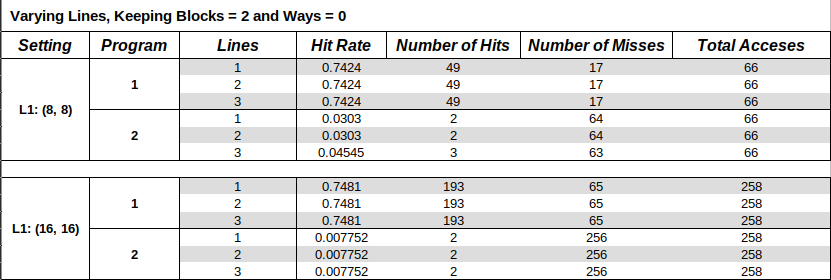
\includegraphics[width=0.8\textwidth]{1.1.png}
  %\caption{\large Performance Parameters}
  \label{fig:example}
\end{figure}
\noindent
\textbf{\large{Inference :}}\\
\begin{enumerate}[label=\alph*)]
  \item Program 1: The number of lines doesn't significantly impact the hit rate. This is because the memory access exhibits contiguous increasing spatial locality.
  \item Program 2: A slight impact is observed on the hit rate, reducing the number of collisions.
\end{enumerate}
\smallskip

\subsection{Variation with Blocks :}
\begin{figure}[H]
  \centering
  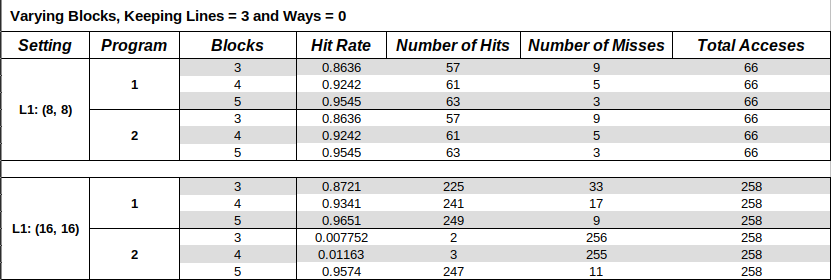
\includegraphics[width=0.8\textwidth]{1.2.png}
  %\caption{\large Performance Parameters}
  \label{fig:example}
\end{figure}
\noindent
\textbf{\large{Inference :}}\\
\begin{enumerate}[label=\alph*)]
  \item Program 1: Larger block size increases the hit rate due to contiguous memory access.
  \item Program 2: Larger block size enhances hit rate by increasing the chances of the requested word being present in the cache.
\end{enumerate}
\textbf{\large{Note :}}\\
In the latter setting for program 2, the hit rate jumps suddenly due to the huge increase in block size and increased spatial locality.
\smallskip

\subsection{Variation with Ways :}
\begin{figure}[H]
  \centering
  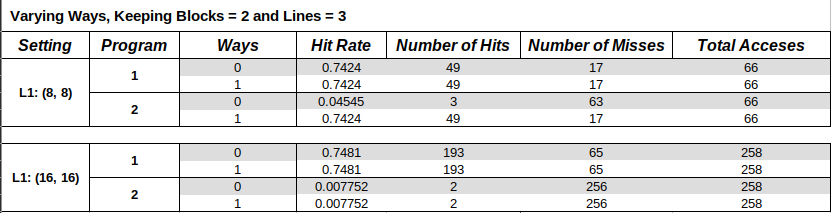
\includegraphics[width=0.8\textwidth]{1.3.png}
  %\caption{\large Performance Parameters}
  \label{fig:example}
\end{figure}
\noindent
\textbf{\large{Inference :}}\\
\begin{enumerate}[label=\alph*)]
  \item Program 1: The number of ways doesn't significantly affect the hit rate, as once a block is exhausted, it is not accessed again.
  \item Program 2: Increases the hit rate by utilizing data fetched in the past, taking advantage of the temporal locality of the program.
\end{enumerate}
\smallskip

\section{Question 2 :}
\begin{figure}[H]
  \centering
  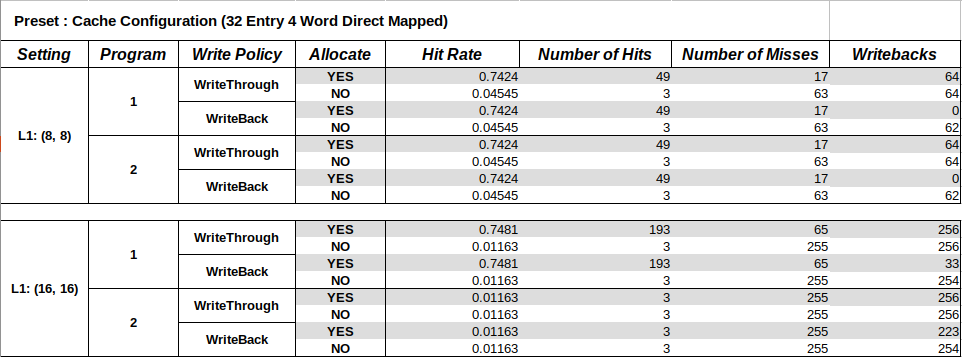
\includegraphics[width=0.8\textwidth]{2.png}
  %\caption{\large Performance Parameters}
  \label{fig:example}
\end{figure}
\noindent
\textbf{\large{Inference :}}\\
\begin{enumerate}[label=\alph*)]
  \item Program 1: Allocation allowed increases the number of hits compared to when disallowed, regardless of the policy. This is because the block is allocated in the cache on a miss, increasing subsequent hits due to increased spatial locality.
  \item Program 2: In the former setting, the above logic applies. However, in the latter setting, the data is too large to benefit from spatial locality before it can be accessed again; it's replaced by another block due to collisions.
\end{enumerate}
\smallskip

\section{Question 3 :}
\begin{figure}[H]
  \centering
  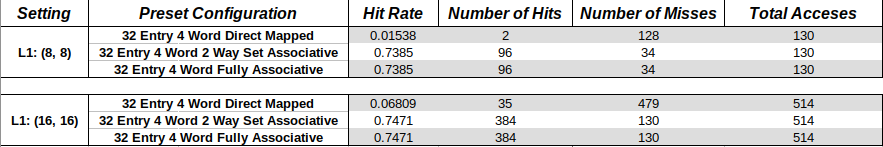
\includegraphics[width=0.8\textwidth]{3.png}
  %\caption{\large Performance Parameters}
  \label{fig:example}
\end{figure}
\noindent
\textbf{\large{Inference :}}\\
As the data is the same, having more ways would be beneficial, allowing retention of older blocks and possibly taking advantage of any temporal locality the program may have.
\smallskip

\end{document}

